\documentclass[12pt,a4paper]{article}

\usepackage[utf8]{inputenc}
\usepackage[T1]{fontenc}
\usepackage[ngerman]{babel}

\usepackage[a4paper,
            left=2.5cm,
            right=2.5cm,
            top=2cm,
            bottom=2cm]{geometry}

\usepackage{lmodern}
\usepackage{parskip}
\usepackage{graphicx}
\usepackage{amsmath}
\usepackage{amssymb}

\newcommand{\R}{\mathbb{R}}


\begin{document}

\begin{center}

    
\includegraphics[width=0.5\textwidth]{../Titlepage/logo.png}\\[1cm]

    {\Large\textbf{Masterarbeitskolloquium}}\\[0.8cm]

    \rule{\textwidth}{0.5pt}\\[0.5cm]

    \LARGE
    \textbf{Kreisbündel mit positiver Skalarkrümmung}\\[0.1cm] 
    \textbf{über vergrößerbaren Mannigfaltigkeiten}\\[0.2cm]

    \rule{\textwidth}{0.5pt}

\end{center}

\vspace{0.5cm}

\begin{center}
    {\Large\textbf{Abstract}}
\end{center}

\vspace{0.3cm}

Wie man dem Titel bereits entnehmen kann ist das Thema meiner Masterarbeit in dem größeren Gebiet der \textit{Skalarkrümmungsgeometrie} angesiedelt. Für eine Riemannsche Mannigfaltigkeit $(M,g)$ ist die Skalarkrümmung eine glatte Funktion $\mathrm{scal}_g \colon M \to \R$. Grob gesprochen misst der Wert $\mathrm{scal}_g(x)$ an einem Punkt $x \in M$, um wie viel das Volumen eines kleinen Balles $B_r(x) \subseteq M$ in $M$ von Radius $r$ um den Punkt $x \in M$ von dem Volumen des gewöhnlichen euklidischen Balls $B_r^\mathrm{eukl.}(0) := \{x \in \R^n \mid ||x|| \leq r\} \subseteq \R^n$ vom selben Radius abweicht. Ist $\mathrm{scal}_g(x) > 0$, so ist das Volumen des Balls in $M$ kleiner als das des entsprechenden euklidischen Balls, ist $\mathrm{scal}_g(x) < 0$ ist es größer und für $\mathrm{scal}_g(x) = 0$ sind diese gleich. 

\begin{center}
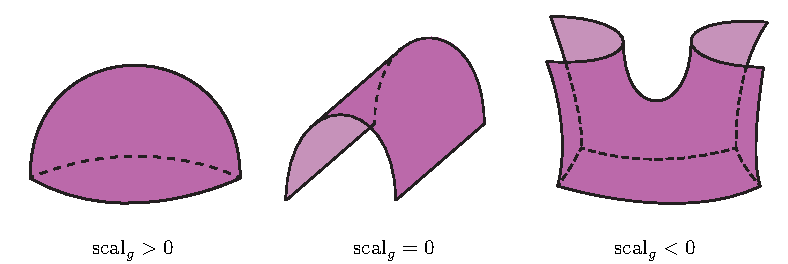
\includegraphics[width=0.9\textwidth]{../graphics/scalar_curvature.pdf}
\end{center}

Wie vieles im Leben beginnt auch meine Masterarbeit zu diesem Thema mit einer Frage von Gromov:

\vspace{0.15cm}

\begin{center}
\begin{minipage}{0.8\textwidth}
    \centering \itshape
    Ist der Totalraum eines Kreisbündels $E \to M$ über einer vergrößerbaren Mannigfaltigkeit $M$ ebenfalls immer vergrößerbar?
\end{minipage}
\end{center}

\vspace{0.15cm}

Es stellt sich raus, dass die Antwort auf diese Frage \textit{nein} ist und sehr konkrete Gegenbeispiele existieren. In meinem Kolloquium möchte ich die darin vorkommenden Begriffe anschaulich erklären und anschließend eine Skizze zur Konstruktion von Gegenbeispielen geben.

\vfill

\textbf{Wann? Wo?:} Montag 21. September, 14:00 Uhr, Raum ?



\end{document}